\documentclass[12pt]{article}

\usepackage[utf8]{inputenc}
\usepackage[T1]{fontenc}
\usepackage{datetime}
\usepackage[spanish]{babel}
\usepackage{graphicx}
\usepackage{listings}
\usepackage{caption}
\usepackage{subcaption}
\usepackage[right=2cm,left=2cm,top=2cm,bottom=2cm]{geometry}
\usepackage{hyperref}
\usepackage{fancyhdr}
\usepackage{color}
\usepackage[export]{adjustbox}
\usepackage{graphicx}
\usepackage{float}
\usepackage{changepage}
\usepackage{multicol}
\usepackage{imakeidx}
\usepackage{csquotes}
\usepackage{array}
\usepackage{tabularx}
\usepackage{xcolor}
\usepackage[backend=biber]{biblatex}
\addbibresource{webgrafia.bib}

\pagestyle{fancy}
\renewcommand{\footrulewidth}{0.4pt}
\setlength{\headheight}{15pt}


\fancyhead[L]{ CEIABD – SBD }
\fancyhead[R]{ Páez Anguita, Víctor }
\fancyfoot[L]{IES Gran Capitán}


\begin{document}

\begin{titlepage}
    \begin{center}
      \Large \bfseries{}
    \end{center}
    \vspace{0.1cm}
    \begin{center}
      \Large \bfseries{}
    \end{center}
    \vspace{0.1cm}
    \begin{center}
     \Large \bfseries{Estructuración de datos}
    \end{center}
    \vspace{0.0001cm}
    \begin{center}
        Departamento de informática \\ I.E.S. Gran Capitán - Córdoba
    \end{center}
        \vspace{2 cm}
\begin{figure}[h!]
    \centering
    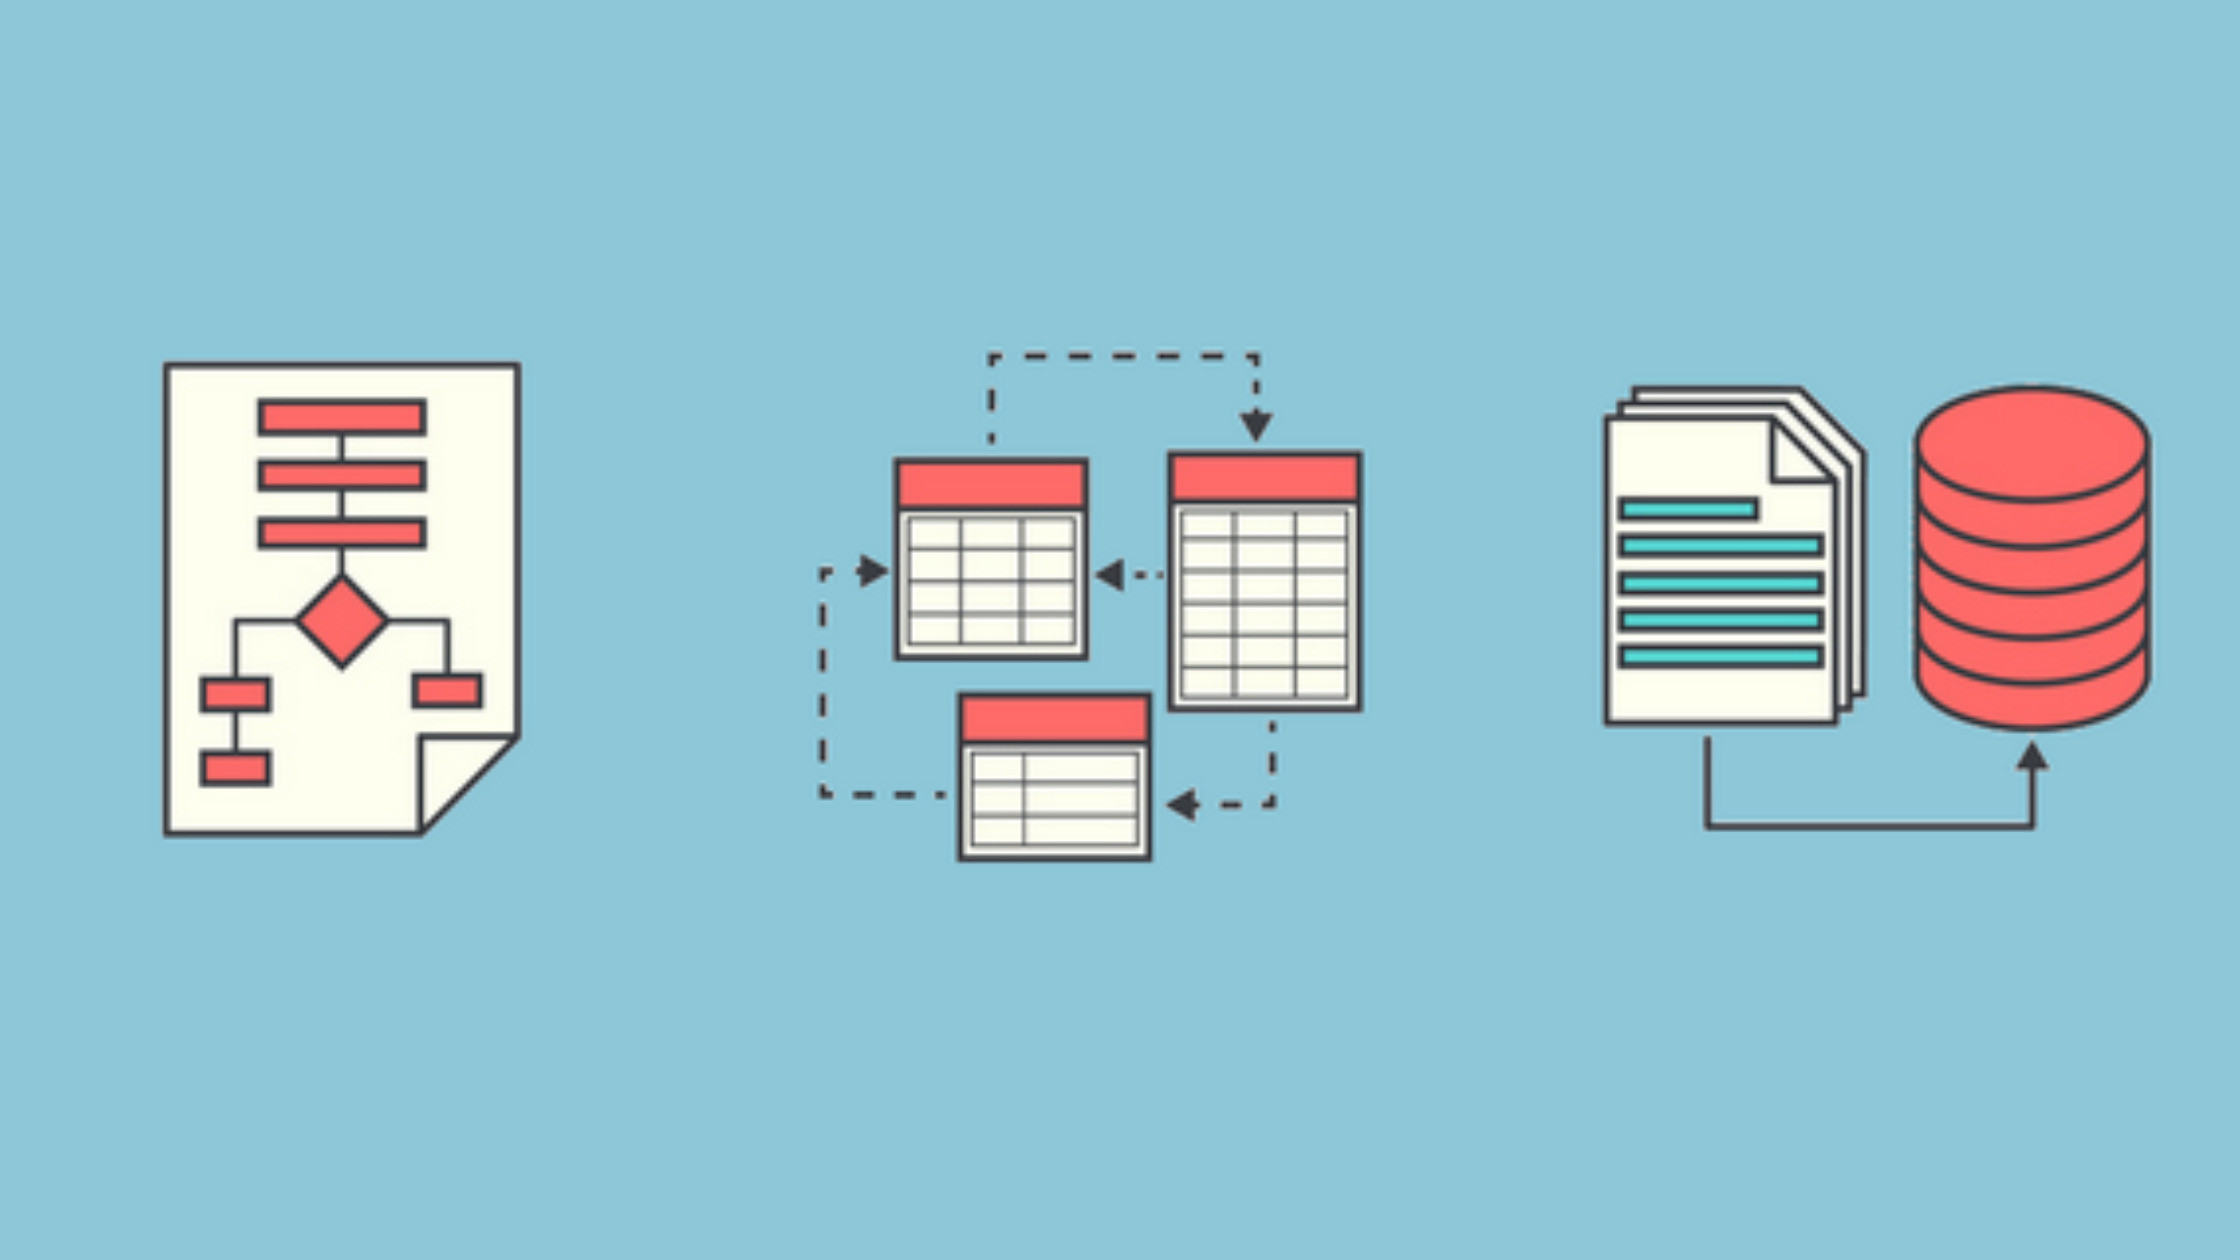
\includegraphics[width=.6\textwidth]{portada.jpg}
    \label{fig:my_label}
\end{figure}
    \vspace{0.2 cm}
    \begin{center}
        Inteligencia artificial y Big data \\ \today 
    \end{center}
    \vspace{4 cm}
\null\hfill \textbf{Desarrollado por:}
\\
\\
\null\hfill Víctor Páez Anguita
\clearpage
\end{titlepage}

%%%%%%%%%%%%%%%%%%%%%%%%%%%Index%%%%%%%%%%%%%%%%%%%%%%%%%%%%%%%%
\tableofcontents
\clearpage
%%%%%%%%%%%%%%%%%%%%%%%%%%%Index%%%%%%%%%%%%%%%%%%%%%%%%%%%%%%%%


\section{Ejemplo de la vida real de la transformación de datos en conocimiento}


\clearpage
\section{Diferencias entre un data lake y un data warehouse}

\renewcommand{\arraystretch}{2} % Espaciado vertical en las celdas

\begin{tabularx}{\textwidth}{|>{\raggedright\arraybackslash}X|>{\raggedright\arraybackslash}X|>{\raggedright\arraybackslash}X|>{\raggedright\arraybackslash}X|}
    \hline
    \textbf{Tipo} & \textbf{Procesamiento por Lotes} & \textbf{Procesamiento en Streaming} & \textbf{Procesamiento en Tiempo Real} \\
    \hline
    \textbf{Latencia} & Alta (puede tardar minutos, horas o más). & Media (procesa datos casi en tiempo real, pero con un pequeño retraso) & Muy baja (milisegundos o menos) \\
    \hline
    \textbf{Frecuencia de actualización} & Periódica (procesos programados) & Continua (procesa datos a medida que llegan) & Instantánea (procesa cada evento al momento)\\
    \hline
    \textbf{Volumen de datos} & Grandes volúmenes procesados en conjunto & Flujo constante de datos & Flujo constante de datos \\
    \hline
    \textbf{Aplicaciones recomendadas} & -Generación de informes -Investigación Médica  -Tareas programables & -Análisis de datos en tiempo casi real -Detección de anomalías -Transmisiones en vivo & -Vigilancia de fraudes -Control de maquinaria -Juegos interactivos \\
    \hline
    \textbf{Ventajas} & -Eficiencia en el uso de recursos -Procesar grandes cantidades de datos & -Proporciona resultados en tiempo cercano al real -Manejo continuo de datos & -Respuesta inmediata -Ideal para decisiones críticas \\
    \hline
    \textbf{Limitaciones} & -No apto para aplicaciones sensibles al tiempo -Retraso entre la recopilación y el análisis de datos &  -Requiere más recursos que el procesamiento por lotes -Puede tener mayor latencia que el tiempo real & -Complejidad técnica -Alto costo de implementación y mantenimiento \\
    \hline
\end{tabularx}

\clearpage

\section{ejemplo real de los 4 tipos de analítica}

\subsection{descriptiva}
\subsection{diagnóstica}
\subsection{predictiva}
\subsection{prescriptiva}


\section{Ejemplo real de catastrofe por culpa del big data con el bussines intelligence}

\section{Relación entre el big data y el bussines intelligence}

\section{Ofertas de trabajo para data science y sus requisitos}

\section{3 busquedas en google con operadores que no conocias}

\section{Analisis de sentimiento}


\clearpage

\section{Bibliografia}

\cite{Estructuracion_de_datos}

\printbibliography

\end{document}
